\chapter{磁盘完成请求时怎样唤醒线程}

启动阶段可以轮询 ATA，运行期的线程却不应一直占着 CPU。请求提交后，IRQ14
报告完成，PIT 提供超时，等待者只能由其中一个结果唤醒。页面、块缓存和设备
FLUSH 还要区分“已修改”“正在写回”和“已经稳定”。

\chapterroute{用户字节的十步路径 $\rightarrow$ ATA 寄存器 $\rightarrow$
IRQ14 与超时竞争 $\rightarrow$ 写回状态 $\rightarrow$ 失败注入。}

\section{用户字节跨重启的完整路径}

write 返回、同次启动读回、块缓存标为 clean 和新机器进程重新读回，是四个不同
强度的结论。只有数据经过系统调用、文件对象、文件系统、缓存写回、ATA PIO 和
FLUSH，并由一个全新的 QEMU 进程重新 mount 后得到相同字节，才形成当前项目的
跨启动持久化证据。

\begin{sidewaysfigure}[p]
  \centering
  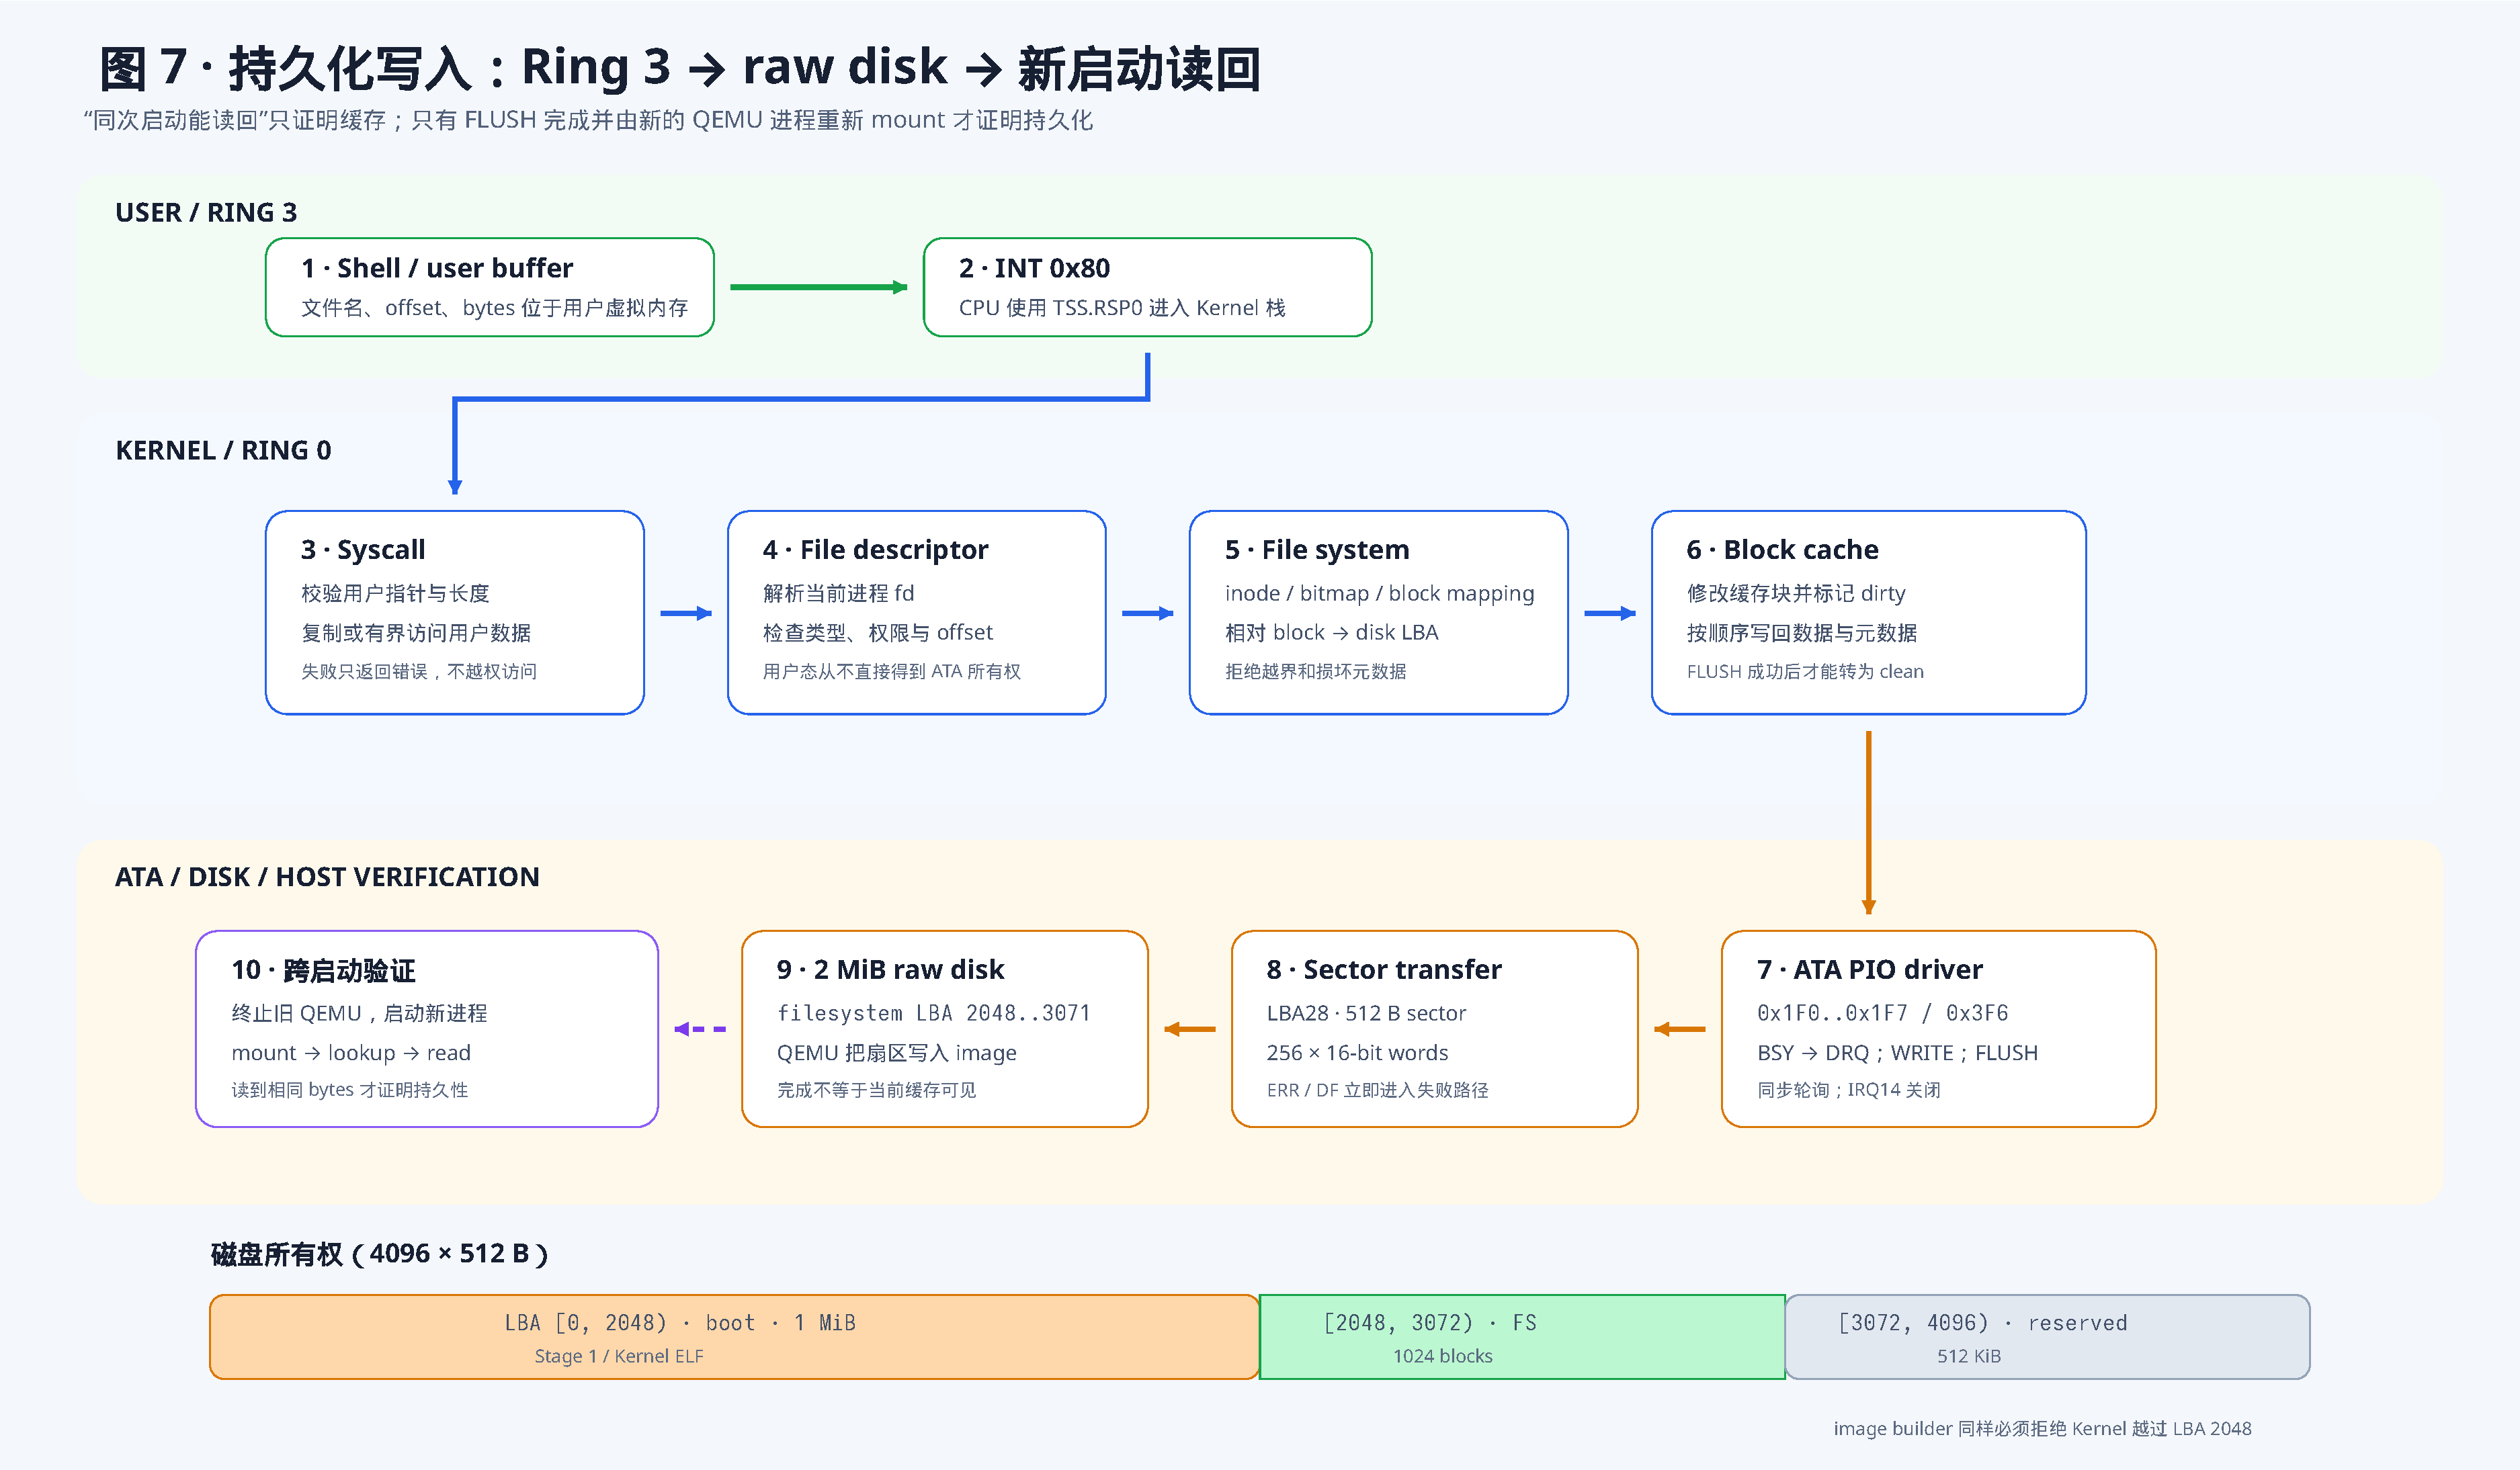
\includegraphics[width=0.96\textheight,height=0.82\textwidth,keepaspectratio]
    {figures/system_wiring/storage_persistence.pdf}
  \caption{Ring 3 文件写入到 raw disk、再由新 QEMU 启动读回的完整矢量路径。
  绿线表示用户请求，蓝线表示内核对象与数据流，橙线表示 ATA/磁盘传输，紫线
  表示跨进程验证；下方同时给出 4096 个扇区的磁盘所有权分区。}
  \label{fig:storage-persistence-full}
\end{sidewaysfigure}
\clearpage

\topic{一、先区分“可见”“已写回”和“持久”}\par
\begin{osgridlongtable}{L{0.20\linewidth}L{0.29\linewidth}L{0.31\linewidth}L{0.10\linewidth}}
结论 & 已经证明 & 还没有证明 & 强度 \\ \hline
write 返回成功 & 内核接受请求并按接口完成当前提交点 & 数据已离开全部 volatile cache & 低 \\ \hline
同次启动读回相同 & 当前内核路径能从缓存或磁盘返回字节 & 重启后仍存在 & 较低 \\ \hline
ATA WRITE 完成 & 控制器接受/处理数据传输 & 设备内部易失缓存已稳定落介质 & 中 \\ \hline
FLUSH 成功 & 设备按当前 ATA 协议完成缓存刷新 & 新启动的 mount/读取逻辑也正确 & 较高 \\ \hline
新 QEMU 进程读回 & 旧进程和所有 Guest RAM 已消失，镜像重新挂载后字节一致 & 任意断电点都有日志级原子恢复 & 当前最强 \\ \hline
\end{osgridlongtable}

\term{持久性}{persistence}表示状态在产生它的执行实例结束后仍可恢复；
\term{耐久性}{durability}通常强调已经承诺成功的数据在规定故障模型下不会
丢失。当前项目检查正常 FLUSH 后跨 QEMU 进程保存；写到任意中间位置突然
断电的恢复由后文 journal、写序和 replay 实验覆盖。

\topic{二、步骤 1--3：用户地址必须在边界上重新验证}
Shell 的文件名、offset 和 bytes 位于用户虚拟地址空间。用户程序执行
\code{INT 0x80} 后，CPU 按 IDT gate 与 TSS.RSP0 切入当前进程的 Ring 0 栈。
硬件只完成特权和栈转换，不会替 Kernel 判断指针安全。

系统调用层必须同时检查：

\begin{itemize}[leftmargin=2em]
  \item 系统调用号存在，参数个数和宽度符合 ABI；
  \item 用户地址处于允许范围，地址加长度不溢出；
  \item 每个跨页范围都具有用户访问和所需读/写权限；
  \item 字符串有最大长度和终止边界，不能无限扫描；
  \item 复制失败只返回确定错误，不把半写内核状态提交给下一层。
\end{itemize}

Kernel 不应在持有可能阻塞其他路径的锁时直接访问可故障用户页。当前模型虽比
完整 demand paging 简单，仍应维持“验证/复制用户数据”与“修改持久对象”的
清楚提交顺序。

\topic{三、步骤 4：fd 不是 inode，也不是磁盘地址}
\term{file descriptor}{文件描述符，fd}只是当前进程 FileTable 中的整数索引。
FileTable 项引用 KernelObject；文件类型进一步引用共享 FileDescription，
后者保存打开状态和当前 offset；文件系统对象再关联 inode。多层间接让复制 fd
可以共享 offset，而两次独立 open 可以得到不同 offset。

\[
\mathrm{fd}
\rightarrow \mathrm{FileTable\ entry}
\rightarrow \mathrm{KernelObject}
\rightarrow \mathrm{FileDescription}
\rightarrow \mathrm{inode/file}.
\]

每一箭头都带引用和权限语义。关闭 fd 只删除当前表项并释放相应引用；只有最后
引用离开时对象才析构。把 fd 数字直接当 inode 编号，会破坏跨进程共享、类型
检查和生命周期。

\topic{四、步骤 5：文件系统把名字和 offset 变成磁盘块}
\term{inode}{索引节点}保存文件类型、大小和数据块映射；
\term{bitmap}{位图}用 bit 记录 inode 或 block 是否已占用；
\term{directory entry}{目录项}把名称关联到 inode；
\term{superblock}{超级块}冻结磁盘格式、范围和校验。一次路径解析依次读取
目录项和 inode，文件 offset 再映射到相对 block，最后加上文件系统分区起点
得到全盘 LBA。

这些结构使用显式小端编码，不能把编译器内存中的 C++ struct 原样写盘。结构体
可能包含 padding、不同对齐或宿主字节序；磁盘格式必须对每个字段宽度、偏移、
合法范围和校验和负责。

\topic{五、步骤 6：block cache 为什么需要 dirty/clean 状态}
块缓存保留近期磁盘块的 RAM 副本，避免每次读写都发 ATA 命令。
\term{dirty}{脏}表示 RAM 副本比持久介质更新；
\term{clean}{干净}表示该副本与已确认的介质状态一致。把内存改完不应立即标
clean；只有数据、元数据按协议写出并完成必要 FLUSH，才能推进状态。

写回次序会影响故障后可解释性。若目录项先指向尚未写好的 inode，或 inode
先指向尚未分配/写好的数据块，断电后会出现悬空引用。当前固定布局使用明确的
Dirty/Clean 提交和全盘一致性检查；更完整的 v2 方案用 ordered metadata
journal 进一步定义崩溃恢复边界。

\topic{六、步骤 7--8：ATA PIO 把一个扇区变成 256 个 word}
驱动向 primary ATA 的任务文件寄存器写 LBA28、扇区数和命令，轮询 BSY、DRQ、
ERR 与 DF。数据口 \code{0x1F0} 按 16 位访问，一个 512 B 扇区需要传输
256 个 word。控制寄存器和状态寄存器仍按 8 位访问，不能为了循环方便把整组
端口都改成同一宽度。

\term{sector}{扇区}是当前 ATA 传输的 512 B 单位；
\term{LBA}{Logical Block Address}是扇区编号；
\term{filesystem block}{文件系统块}是文件系统分配和缓存单位。当前图中两者
同为 512 B，概念仍不能合并，因为未来文件系统可用多个 sector 组成一个 block，
NVMe 也有自己的 namespace 与 logical block 规格。

\topic{七、步骤 9：raw disk 是镜像容器，不等于文件系统}
\term{raw disk image}{原始磁盘镜像}按扇区保存整块虚拟磁盘，没有宿主文件系统
替 Guest 自动解释内容。v0.11 的历史 2 MiB 镜像共有
\[
4096\times512\ \mathrm{B}=2\ \mathrm{MiB}.
\]

\begin{osgridlongtable}{L{0.22\linewidth}L{0.22\linewidth}L{0.25\linewidth}L{0.21\linewidth}}
LBA 半开区间 & 大小 & 所有者 & 内容 \\ \hline
\([0,2048)\) & 1 MiB & 启动镜像布局 & Stage 1、Kernel 容器/ELF 与保留结构 \\ \hline
\([2048,3072)\) & 512 KiB & 文件系统 & 1024 个当前文件系统块 \\ \hline
\([3072,4096)\) & 512 KiB & 明确保留 & 不允许 Kernel 镜像或文件系统越界占用 \\ \hline
\end{osgridlongtable}

半开区间让长度等于 end-start，相邻区域可以无歧义拼接。镜像构建器和 Kernel
都必须拒绝越过边界；否则一次大文件写入可能覆盖下一次启动所需的 Kernel，
表面文件系统成功却让机器再也不能启动。

自 v1.6 起镜像已扩为逻辑 1 GiB 稀疏文件；v1.9 当前从 LBA 32768 起分配
固定 256 MiB rootfs。本表保留为第一版持久格式的历史基线，详细新布局见本章
后续 rootfs v2 节。

\topic{八、步骤 10：为什么必须终止旧 QEMU}
如果只在同一个 Guest 中 unmount/mount 或重新读取，RAM 中仍可能保留缓存、
对象和错误的未写回副本。自动测试先等待写入、sync 和成功标记，再终止旧 QEMU
进程；随后用同一磁盘文件启动全新的 QEMU。新 Guest 的 CPU、RAM、Kernel 堆和
块缓存均重新建立，只能从 disk image 读取状态。

新启动必须通过 superblock 验证、mount、路径查找、inode/block 读取，最终得到
精确相同字节。测试还要使用禁止标记确保没有悄悄格式化损坏磁盘、没有走错误
恢复分支，超时则视为失败而非“可能还在写”。

\topic{九、把 QEMU ATA 换成实体 NVMe 时哪些层保持}
文件描述符、FileDescription、路径、inode、bitmap、块缓存和大部分文件系统
规则可以保持；最下层块设备驱动和发现路径必须替换。DFR1142 的 M.2 M Key
连接 PCIe x1，常见 SSD 使用 NVMe，而当前 STUOS 只驱动 QEMU 的 legacy ATA
PIO。实体适配至少还需：

\begin{enumerate}[leftmargin=2.2em]
  \item 通过 UEFI/ACPI/PCIe 配置空间发现 root 与 NVMe function；
  \item 分配/读取 BAR，把控制器 MMIO 映射成正确缓存属性；
  \item 建立 admin/I/O submission 与 completion queue；
  \item 为队列和数据准备 DMA 可见物理内存，处理 doorbell 与完成中断/轮询；
  \item 把 NVMe namespace block 接到现有 BlockDevice 抽象，并重新验证
        FLUSH/持久性语义。
\end{enumerate}

所以“载板有 M.2”只证明物理插槽和 PCIe 通道存在；“Kernel 有文件系统”只证明
上层格式和对象模型存在。中间 PCIe/NVMe 驱动链没有实现时，两端不能自动接通。

\topic{十、失败现象怎样对应到十步链}\par
\begin{osgridlongtable}{L{0.25\linewidth}L{0.31\linewidth}L{0.34\linewidth}}
现象 & 最可能边界 & 应保存的证据 \\ \hline
write 立即返回参数错误 & 用户复制、fd 类型/权限或范围检查 & syscall 号、fd、长度、精确错误码 \\ \hline
同次读回正确、重启丢失 & dirty cache、ATA WRITE/FLUSH 或镜像绑定 & dirty/clean 计数、状态位、FLUSH 标记 \\ \hline
重启后自动格式化 & mount 的全零/损坏分类错误 & superblock 原始字节、CRC、禁止标记 \\ \hline
小文件正常、大文件破坏启动 & block/LBA 边界或长度溢出 & 目标半开区间、镜像审计、受影响 LBA \\ \hline
第二次 QEMU 读到旧内容 & 旧进程未终止、磁盘文件错误或 flush 未完成 & 进程边界、镜像路径/hash、完成标记 \\ \hline
随机卡在 ATA & BSY/DRQ/ERR/DF 轮询与预算 & 最后状态、命令、LBA、剩余 timeout \\ \hline
\end{osgridlongtable}

端到端测试证明整条链能协作，单元/随机测试则分别证明路径解析、位图、cache、
fd 和状态机边界。两者不能互相替代：只跑 QEMU 很难覆盖每个损坏字段，只跑
内存模型又不能证明真实 ATA 端口和跨启动镜像。

\section{磁盘完成请求时怎样唤醒 Thread}

异步 I/O 把命令、缓冲区、完成结果和等待者从调用栈中抽出来，交给一个在
IRQ、超时和取消竞争下仍只有唯一结论的请求状态机。可写共享映射也不能只打开
PTE 的 W 位；Kernel 必须先取得脏页
责任，写回时重新建立下一次写通知边界。

\topic{为什么启动链必须轮询，运行期才适合中断}
CPU 从复位向量进入 ROM 时没有 Process、Thread、IDT、PIC 路由、WaitQueue
或 scheduler。ROM 为了读取 Stage 1，只能发出 ATA 命令，再有界检查
BSY、DRQ、ERR 和 DF。Stage 1 也不能等待由尚未装载的 Kernel 处理 IRQ。
因此 polling 是启动依赖图的必然结果，不是尚未学会中断的临时错误。

\begin{lstlisting}
Reset ROM
  -> bounded ATA polling
  -> load Stage 1
  -> bounded ATA polling
  -> load Kernel
  -> IDT + PIC + PIT + scheduler + WaitQueue
  -> IRQ14 completion becomes safe
\end{lstlisting}

运行期继续轮询却会浪费已经存在的并发结构。一个 Thread 等设备时反复读端口，
其他 Ready Thread 无法获得本应可用的 CPU。v1.16 因而保留两种适配器：
ROM、Stage 1 和 early Kernel 以 nIEN 禁止设备中断并有界轮询；调度器就绪后，
运行期请求队列才清 nIEN、开放 IRQ14。两者不能同时拥有 ATA 通道。

早期 PATA 控制器与现代 NVMe 的另一个差别是：legacy primary channel 没有
command tag。IRQ14 本身不会携带“这是第几个请求”。只要硬件里同时存在多个
未完成命令，软件便无法可靠配对。因此软件队列可以有多个 Queued，请求进入
硬件后却只能有一个 Issued。这个单飞约束来自协议，不是数组容量不够。

\topic{从 ATA 引脚语义到 CPU vector 0x2E}
QEMU 的 \code{pc} 机器模拟传统连线。primary ATA controller 把中断接到
slave 8259A 的 IR6；slave 的输出接到 master IR2；master INTR 再经 Local
APIC LINT0 的 ExtINT virtual-wire 模式到达 CPU。

\begin{pdfdiagram}[node distance=8mm and 10mm]
  \node[os hardware] (ata) {ATA primary\\IRQ14};
  \node[os hardware,right=of ata] (slave) {8259A slave\\IR6};
  \node[os hardware,right=of slave] (master) {8259A master\\IR2 cascade};
  \node[os hardware,right=of master] (lapic) {LAPIC LINT0\\ExtINT};
  \node[os state,below=of lapic] (cpu) {CPU vector 0x2E\\IDT interrupt gate};
  \node[os state,left=of cpu] (asm) {NASM IRQ stub\\统一 176 B frame};
  \node[os block,left=of asm] (cpp) {InterruptRuntime\\ATA completion};
  \draw[os arrow] (ata) -- (slave);
  \draw[os arrow] (slave) -- (master);
  \draw[os arrow] (master) -- (lapic);
  \draw[os arrow] (lapic) -- (cpu);
  \draw[os arrow] (cpu) -- (asm);
  \draw[os arrow] (asm) -- (cpp);
\end{pdfdiagram}
\diagramnote{IRQ14 经过 slave 与 master 两层 in-service 状态；EOI 必须先 slave 后 master。}

PIC 初始化后全屏蔽。v1.16 最终掩码是 \code{0xBFF8}：

\begin{table}[htbp]
\centering
\small
\begin{osgridtabularx}{\textwidth}{l l X}
控制器 & mask & 开放输入\\ \hline
master & \code{0xF8 = 11111000b} & IRQ0 PIT、IRQ1 keyboard、IRQ2 cascade\\ \hline
slave & \code{0xBF = 10111111b} & IR6，即系统 IRQ14\\ \hline
\end{osgridtabularx}
\caption{开放 slave IRQ 必须同时开放 master cascade}
\end{table}

若只清 slave bit 6，slave 可以登记 in-service，但 master 仍挡住级联；若只清
master bit 2，级联线可达，却没有允许的 slave 来源。真实 IRQ14 完成后先向
\code{0xA0} 发 EOI，再向 \code{0x20} 发 EOI；相反顺序可能让级联服务状态
停留，下一次 IRQ 看起来像随机丢失。

\topic{ATA 命令块、状态位与控制位}\par
\begin{table}[htbp]
\centering
\small
\begin{osgridtabularx}{\textwidth}{l l l X}
端口 & 宽度 & 名称 & 读写语义\\ \hline
\code{0x1F0} & 16 & DATA & 一个扇区 256 个 word\\ \hline
\code{0x1F1} & 8 & ERROR/FEATURES & 读错误，写 feature\\ \hline
\code{0x1F2} & 8 & SECTOR COUNT & 当前命令写一扇区\\ \hline
\code{0x1F3..0x1F5} & 8 & LBA LOW/MID/HIGH & LBA 的低 24 位\\ \hline
\code{0x1F6} & 8 & DRIVE/HEAD & master、LBA mode 与 LBA[27:24]\\ \hline
\code{0x1F7} & 8 & STATUS/COMMAND & 读状态，写命令\\ \hline
\code{0x3F6} & 8 & ALT STATUS/CONTROL & 读状态不确认 IRQ；写 nIEN/SRST\\ \hline
\end{osgridtabularx}
\caption{primary ATA command block 与 control port}
\end{table}

Status 的决定性位如下：

\begin{table}[htbp]
\centering
\small
\begin{osgridtabularx}{\textwidth}{c l X}
位 & 名称 & v1.16 解释\\ \hline
7 & BSY & 设备仍拥有内部状态，不能发下一命令\\ \hline
6 & DRDY & 设备就绪提示，不单独表示传输完成\\ \hline
5 & DF & device fault，本请求完成为 DeviceError\\ \hline
3 & DRQ & CPU 必须执行一个数据阶段\\ \hline
0 & ERR & 命令错误，读取 ERROR 并完成为 DeviceError\\ \hline
\end{osgridtabularx}
\caption{ATA STATUS 标志不是可任意组合的软件布尔量}
\end{table}

Device Control bit 1 是 nIEN，置一禁止设备 IRQ；bit 2 是 SRST。读取普通
status 可能确认 pending interrupt，读取 alternate status 不确认，所以两种
端口不能仅因返回相似字节便互换。

Read 请求收到 DRQ IRQ 后执行 256 次 16-bit IN；Write 在第一个 DRQ IRQ
执行 256 次 16-bit OUT，随后还要等待设备完成 IRQ；Flush 没有数据阶段。
逐 word 传输不打印日志，否则串口开销会改变设备与调度时序。

\topic{RFLAGS.IF 与页故障 error code}
RFLAGS bit 9 的 IF 控制可屏蔽外部中断。Kernel 在 IDT、PIC、设备对象和请求
存储发布前保持 IF=0，全部准备完成后才 STI。interrupt gate 进入时处理器
清 IF，并把旧 RFLAGS 保存进特权帧；IRETQ 恢复它。C++ handler 不在任意点
重新 STI，避免同一单飞请求被嵌套 IRQ 重入。

文件页的第一次写则依赖 vector 14 的 page-fault error code：

\begin{table}[htbp]
\centering
\small
\begin{osgridtabularx}{\textwidth}{c l l X}
位 & 名称 & 写通知要求 & 排除的情况\\ \hline
0 & P & 1 & not-present 首次装页\\ \hline
1 & W/R & 1 & 读访问\\ \hline
2 & U/S & 1 & Kernel 自身访问\\ \hline
3 & RSVD & 0 & 页表保留位损坏\\ \hline
4 & I/D & 0 & 取指权限 fault\\ \hline
\end{osgridtabularx}
\caption{writable FileShared 只接管 present+write+user 保护 fault}
\end{table}

真正只读文件映射继续失败；FilePrivate 进入 COW；FileShared 才进入
MarkDirty。若把所有写 fault 都直接改 PTE.W，便会同时破坏只读保护、private
隔离和 dirty backpressure。

\topic{请求身份为何不能等于数组下标}
\code{BlockRequestQueue} 使用调用方提供的 64 槽固定存储，不在 IRQ 中申请。
每个请求保存 operation、LBA、Kernel buffer、owner Thread、absolute deadline、
state、result 和 64 位单调 identifier。

\begin{lstlisting}
Unused
  -> Queued
       -> Completed(Cancelled)
       -> Issued
            -> Completed(Succeeded)
            -> Completed(DeviceError)
            -> Completed(TimedOut)
  -> Reap -> Unused
\end{lstlisting}

数组下标会复用。若等待者只保存下标，请求 A 完成后槽位立刻给请求 B，迟醒的
等待者可能把 B 当成 A，这就是 ABA。identifier 与槽位分离，通用队列的消费方
必须在复制冻结结果后显式 Reap，槽位才重新成为 Unused。生产 ATA 适配器在
IRQ/超时路径中完成这次 copy+Reap，再把独立完成记录交给调度器；等待 Thread
不引用已经复用的槽位。

Issued 请求不能普通取消。命令已经进入设备，仅从链表删除不会撤回硬件状态；
稍后 IRQ 会被下一请求误认。Queued 可以取消，因为它尚未进入设备。

容量耗尽时 Submit 返回明确失败。队列不能覆盖最旧请求，也不能无限增长。
64 是本阶段的内存/压力边界，identifier 和累计统计仍使用显式 \code{uint64_t}。

\topic{IRQ 与 PIT 超时怎样只产生一个结果}
IRQ14 和 PIT IRQ0 可能在同一 deadline 附近到达。唯一完成由状态转移保证：

\begin{enumerate}
  \item IRQ14 先把 Issued 变为 Completed，PIT 随后看不到可超时的 Issued；
  \item PIT 先提交 TimedOut，迟到 IRQ 不能再次 Complete 同一请求；
  \item 重复解析增加诊断统计，但不能覆盖首次结果。
\end{enumerate}

超时不仅是返回值。ATA 可能仍 BSY、等待 data word 或准备产生迟到 IRQ。
ResolveTimeout 获胜后执行 software reset：

\begin{lstlisting}
Complete(TimedOut)
  -> SRST = 1
  -> required delay reads
  -> SRST = 0
  -> bounded wait for BSY clear
  -> only then IssueNext
\end{lstlisting}

若只唤醒 Thread 就发下一命令，两个协议阶段会交叉，队列在软件上正确而设备
状态已经损坏。若 reset 的有界 BSY 检查也失败，controller 被永久冻结；
队列余项逐个以 DeviceError 完成，后续 Submit 直接失败，不再向未知状态的
硬件发命令。这样等待者能收敛，设备所有权也不会被伪装成已经恢复。

\topic{BlockIo 等待与调度证据}
显式 sync 在写回 VFS 后提交异步 Flush。调用 Thread 以请求 identifier 进入
\code{WaitCondition::BlockIo}。IRQ handler 只把 owner 从 Blocked 变为 Ready，
不在任意 IRQ 调用栈上直接切换；现有返回用户态前调度边界稍后选择它。

\begin{pdfdiagram}[node distance=8mm and 10mm]
  \node[os state] (a) {Thread A\\Submit Flush};
  \node[os state,right=of a] (blocked) {A: Blocked\\BlockIo};
  \node[os block,right=of blocked] (b) {Thread B\\继续前进};
  \node[os hardware,below=of b] (irq) {ATA IRQ14};
  \node[os state,left=of irq] (ready) {copy + Reap\\匹配 owner/id};
  \node[os state,left=of ready] (reap) {A: Ready\\结果写入现场};
  \draw[os arrow] (a) -- (blocked);
  \draw[os arrow] (blocked) -- (b);
  \draw[os arrow] (b) -- (irq);
  \draw[os arrow] (irq) -- (ready);
  \draw[os arrow] (ready) -- (reap);
\end{pdfdiagram}
\diagramnote{OTHER\_THREAD\_PROGRESS=1 证明等待期间发生了真实前进，而不只证明最终返回。}

普通 signal 不把 BlockIo 当成字符输入等待唤醒。若一个系统调用需要可中断 I/O，
必须另行冻结取消、设备撤回和 restart ABI；v1.16 不伪造该语义。

完成路径同时核对 owner Thread 槽和 64 位 identifier。Thread 已退出或槽位已
复用时，迟到完成成为 abandoned 诊断，不会唤醒后来占用同一槽的新 Thread。
当前 rootfs 扇区 Read/Write 仍走有界同步 PIO；本阶段接入 BlockIo 的真实生产
消费者是显式 sync 的最终 ATA FLUSH。异步 Read/Write 状态机是后续迁移
journal 和块消费者的基础，不能据此宣称全部文件 I/O 已异步化。

\topic{为什么 clean/dirty 两态仍然不够}\par
\begin{table}[htbp]
\centering
\small
\begin{osgridtabularx}{\textwidth}{l X l}
状态 & 责任 & 零引用时能否 clean LRU 淘汰\\ \hline
Empty & 没有 frame 或文件身份 & 不适用\\ \hline
Clean & frame 与文件一致，无写回债务 & 可以\\ \hline
Dirty & 内存比文件新 & 不可以\\ \hline
Writeback & writer 正在提交这个快照 & 不可以\\ \hline
Error & 上次 writer 失败，债务仍存在 & 不可以\\ \hline
\end{osgridtabularx}
\caption{Error 不是 Clean，也不是没有诊断信息的 Dirty}
\end{table}

失败时若清 dirty，未落盘数据会被伪装成可淘汰；若只保留一个 dirty bit，又
无法分辨是否已有 writer。显式 Writeback/Error 让失败页保留 frame、identity
与重试责任。

dirty hard limit 在 MarkDirty 之前检查。达到上限，页故障返回失败，PTE 仍
只读。不能先开放 PTE 再发现无容量，否则用户已经能够继续修改，缓存却无法
记录这份债务。

\topic{用写保护捕获 MAP\_SHARED 修改}
x86 没有“每次 store 都调用 Kernel”的页模式。v1.16 使用 write-protect
notification：

\begin{enumerate}
  \item 完整 FileShared 页从 VFS 读入 FilePageCache；
  \item 所有 alias 指向同一 frame，PTE 初始只读；
  \item 第一次用户 store 产生 present+write+user fault；
  \item Kernel 验证 VMA、文件范围和 writable open，执行 Clean 到 Dirty；
  \item 成功后才设置该 PTE.W，并 \code{INVLPG}；
  \item CPU 重试原 store，其他 alias 立即看到共享 frame 的新字节。
\end{enumerate}

fork 不对 FileShared 加 COW，父子仍共享文件页；FilePrivate 继续走 COW，
不会进入文件写回。

sync 开始时必须重新写保护所有 writable FileShared PTE。否则 writer 把页
交给 VFS 后，用户仍能经 writable PTE 修改，而缓存最终被标为 Clean。重新
保护让“写回快照之后的新 store”再次 fault 并形成下一轮 Dirty。

\topic{从页身份到 ATA FLUSH 稳定边界}\par
\begin{lstlisting}
Protect shared writable PTEs
  -> Dirty/Error page Writeback
  -> UserFileBackingManager::WritePage
  -> Vfs::WriteAt(file offset; no fd offset change)
  -> rootfs transaction and BlockCache
  -> Vfs::Sync
  -> asynchronous ATA FLUSH
  -> IRQ14 Succeeded
\end{lstlisting}

文件页 identity 不能使用 fd：fd 可以关闭、duplicate 和复用，映射仍继续存在。
当前 key 使用 mount/superblock identity、inode identifier 与 inode
generation。

rootfs 有两种 generation。transaction generation 描述盘面提交次数，应随
普通写增长；VFS superblock generation 描述一次 mount 的身份，必须保持
稳定。若把前者每次复制给后者，同一 inode 会在一次写前后产生两个 cache key，
shared alias 便不再共享。v1.16 的 rootfs 集成测试专门冻结这条边界。

FLUSH 完成只说明当前设备模型报告先前写入已越过其 cache 边界；v1.17 还需
定义数据、metadata、journal descriptor 和 commit record 的顺序。没有
journal 时，v1.16 仍只能在 Dirty superblock 后拒绝不完整事务，不能自动恢复。

\topic{日志为何必须低频且带两种时间}
ATA status、PIO word、cache lookup、PIT tick 都是热路径。逐次打印会让串口
成为主要工作负载并改变 IRQ 竞争。项目只在初始化、请求提交、唯一完成、
shared writeback 验证和终态统计输出 marker。

\begin{lstlisting}
ATA_IRQ14_READY
ATA_REQUEST_CAPACITY=0x40
FLUSH_SUBMIT_REQUEST
FLUSH_SUBMIT_TIME_NS
COMPLETION_RESULT
COMPLETION_TIME_NS
OTHER_THREAD_PROGRESS
FILE_SHARED_WRITEBACK_VERIFIED
\end{lstlisting}

来宾纳秒来自 PIT，用于 deadline 和顺序；QEMU runner 添加的
\code{[QEMU][T+...ms]} 是宿主收到串口行的单调时间，只用于定位慢阶段。
两种时钟起点和调度环境不同，不能比较绝对值。

\topic{测试怎样覆盖状态而不是只看最终成功}\par
\begin{table}[htbp]
\centering
\small
\begin{osgridtabularx}{\textwidth}{l X}
证据层 & v1.16 覆盖\\ \hline
单元 & 参数、FIFO、单飞、容量、取消、完成、超时、Reap、dirty limit、Error 重试\\ \hline
集成 & completion/timeout 后下一请求、PIC cascade、rootfs identity 稳定\\ \hline
随机 & 两个固定种子模型各 100000 步，逐步对照请求与页状态参考模型\\ \hline
故障 & ATA busy/error/timeout、重复解析、writer 失败与重试\\ \hline
QEMU & 三档 RAM、真实 IRQ14、shared alias、落盘读回、private 隔离与 Thread 前进\\ \hline
\end{osgridtabularx}
\caption{最终出现一行 READY 不能代替中间状态和失败证据}
\end{table}

多个 64 GiB TCG QEMU 并发会竞争宿主 CPU，交互式逐键协议可能超过有限进度
门限。宿主逻辑测试可以并行；交互式、persistence 和 capacity QEMU 在发布时
串行复验，并继续保留有限 timeout。无限等待不能区分“机器慢”和真实死锁。

这次串行复验还抓到一个跨阶段竞态：父 Shell 已发布 foreground PGID 时，
child 可能尚未运行到恢复默认 Ctrl-C/Z disposition，于是控制信号调用从
Shell 继承的 handler。正确修复不是让 QMP 多等一会，而是父进程在 fork 前
屏蔽两种信号；child 先恢复默认 action、加入 PGID，再恢复继承前 mask。
窗口内到达的信号只进入 pending，解除 mask 时才按 child 的默认动作交付。

\topic{本阶段没有宣称什么}\par
\begin{itemize}
  \item ATA 仍是 primary master、LBA28、PIO、单飞，没有 DMA/AHCI/NVMe；
  \item writable shared 暂只接受完整页；
  \item 只有全局显式 sync，没有 \code{msync} 和后台 flusher；
  \item Error 页持续占用 cache 并产生回压，不会静默丢弃；
  \item rootfs 尚无 journal/replay；v1.17 才加入 credits、commit 与断电矩阵；
  \item 单 BSP 下完成状态正确，不宣称已经处理跨 CPU completion 与 cache coherence。
\end{itemize}

这些边界把学习顺序保持清晰：v1.16 先建立“请求只能完成一次、脏页责任不会
消失、写回有真实设备稳定边界”，v1.17 再讨论多块元数据事务怎样在断电后只
恢复为完整旧状态或完整新状态。

